\documentclass[12pt]{article}
 
\usepackage[margin=1in]{geometry} 
\usepackage{amsmath,amsthm,amssymb}
\usepackage{graphicx}
\usepackage{subcaption}
 
\newcommand{\N}{\mathbb{N}}
\newcommand{\Z}{\mathbb{Z}}

\begin{document}
 
%\renewcommand{\qedsymbol}{\filledbox}
 
\title{Assignment 1}
\author{Gabriele Stulzer\\ 
Optimisation-Based Robot Control}
 
\maketitle

\section*{Position Stabilization}
 
\subsection*{Question 1}
\textit{What can you say about the relative performance of the different implementations of IC in the different settings? What is the effect of friction on the performance of the different versions of the IC controller? Report the values of the tracking errors that you got in simulation.}

\begin{figure}[h!]
    \centering
    \begin{subfigure}[b]{0.4\linewidth}
    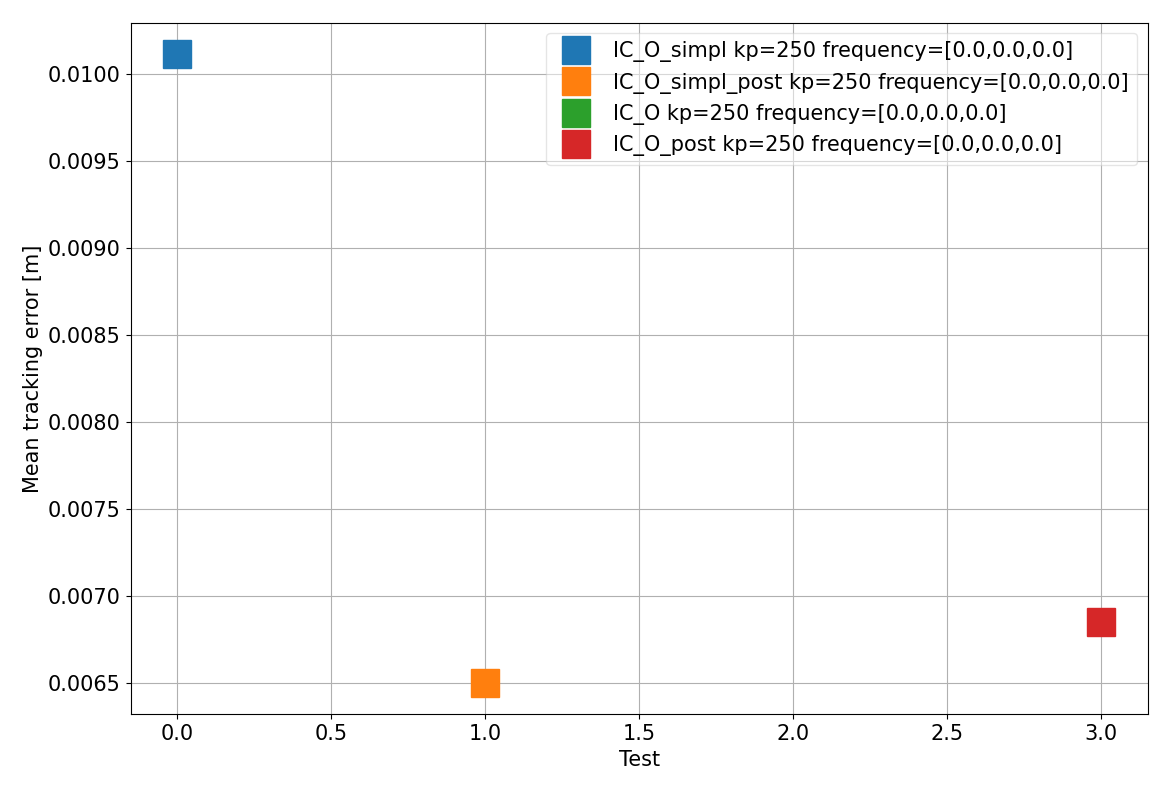
\includegraphics[width=\linewidth]{images/Image1.png}
    \caption{No Friction}
    \end{subfigure}
    \begin{subfigure}[b]{0.4\linewidth}
    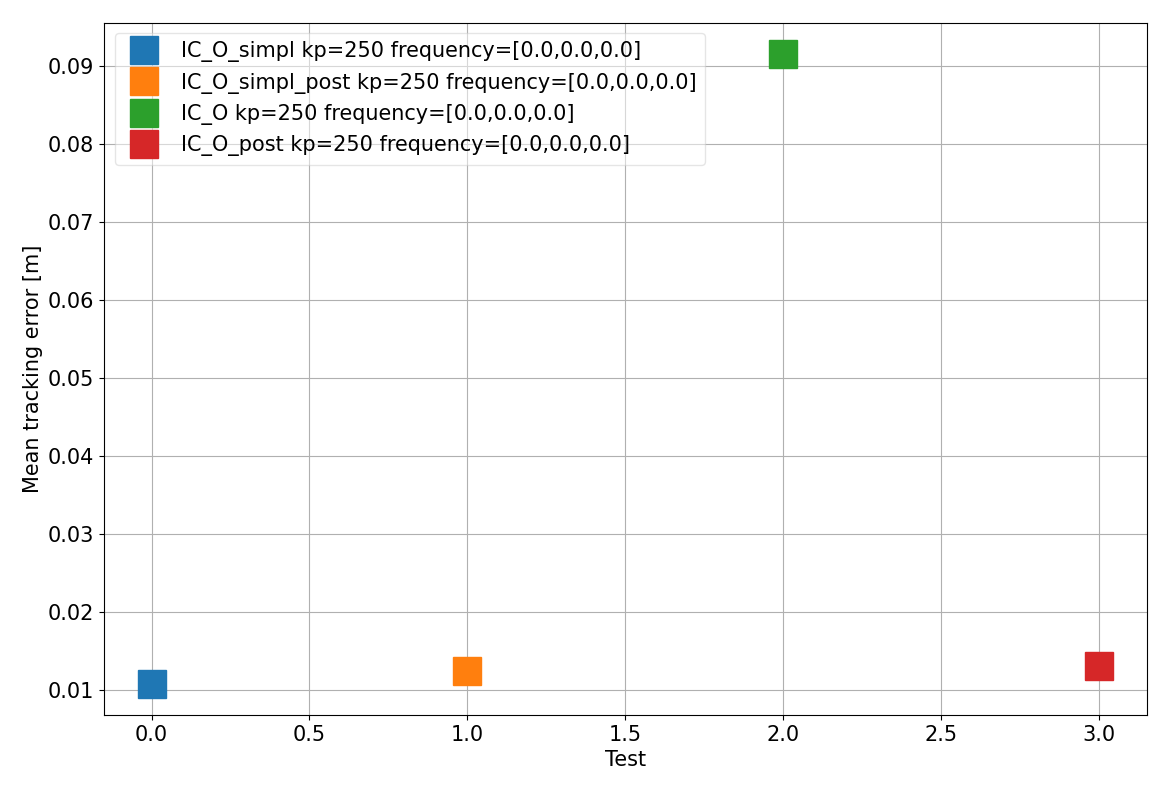
\includegraphics[width=\linewidth]{images/Image2.png}
    \caption{With Friction}
    \end{subfigure}
  \label{fig:psnofriction}
\end{figure}

\paragraph*{}
When considering the performance of the four implementation of Impedance Controller I can clearly see that in some situations we have a good convergence on the joint position and velocities,
and in the case of the full implementation without the secondary task for joint position the joint velocities increase exponentially and diverges to infinity
causing the controller to fail the stabilization on the desired position.

\paragraph*{}
Considering the scenario without friction we can observe that adding the secondary task for joint position, improves drastically the general behavior of the controller,
converging nearly instantaneously to the desired end effector position and keeping a stable position.
Instead, the implementations without secondary task either fail to converge to the desired position or converges with the joints continuously in motion.

\paragraph*{}
Adding the friction for the robot joints improves the performance of the controllers without secondary task, achieving, also with those implementations, a stable joints behavior.

\subsection*{Question 2}
\textit{In one case, a controller fails to stabilize the end effector. In your opinion, why does it happen and why do the other controllers manage to stabilze the desired position?}

\paragraph*{}
In my opinion the implementation of the full version of Impedance Controller fails to stabilize the end effector because it takes into account the factor \(\mu\). Achieving an imprecise compensation of the 
gravitational and centrifugal forces. Instead, in the simplified version we remove the term \(\mu\) for a simplified term \(h\) that reduces the complexity of
the overall controller and introducing a simpler term to converge.


\section*{Trajectory Tracking}
 
\subsection*{Question 1}
\textit{
    What can you say about the relative performance of OSC and IC in the different settings? 
    Which controller performed best at higher frequency of the reference trajectory? 
    How does the relative performance of the controllers varies considering the two frequency values? 
    Report the values of the tracking errors that you got in simulation.
}

\begin{figure}[h!]
    \centering
    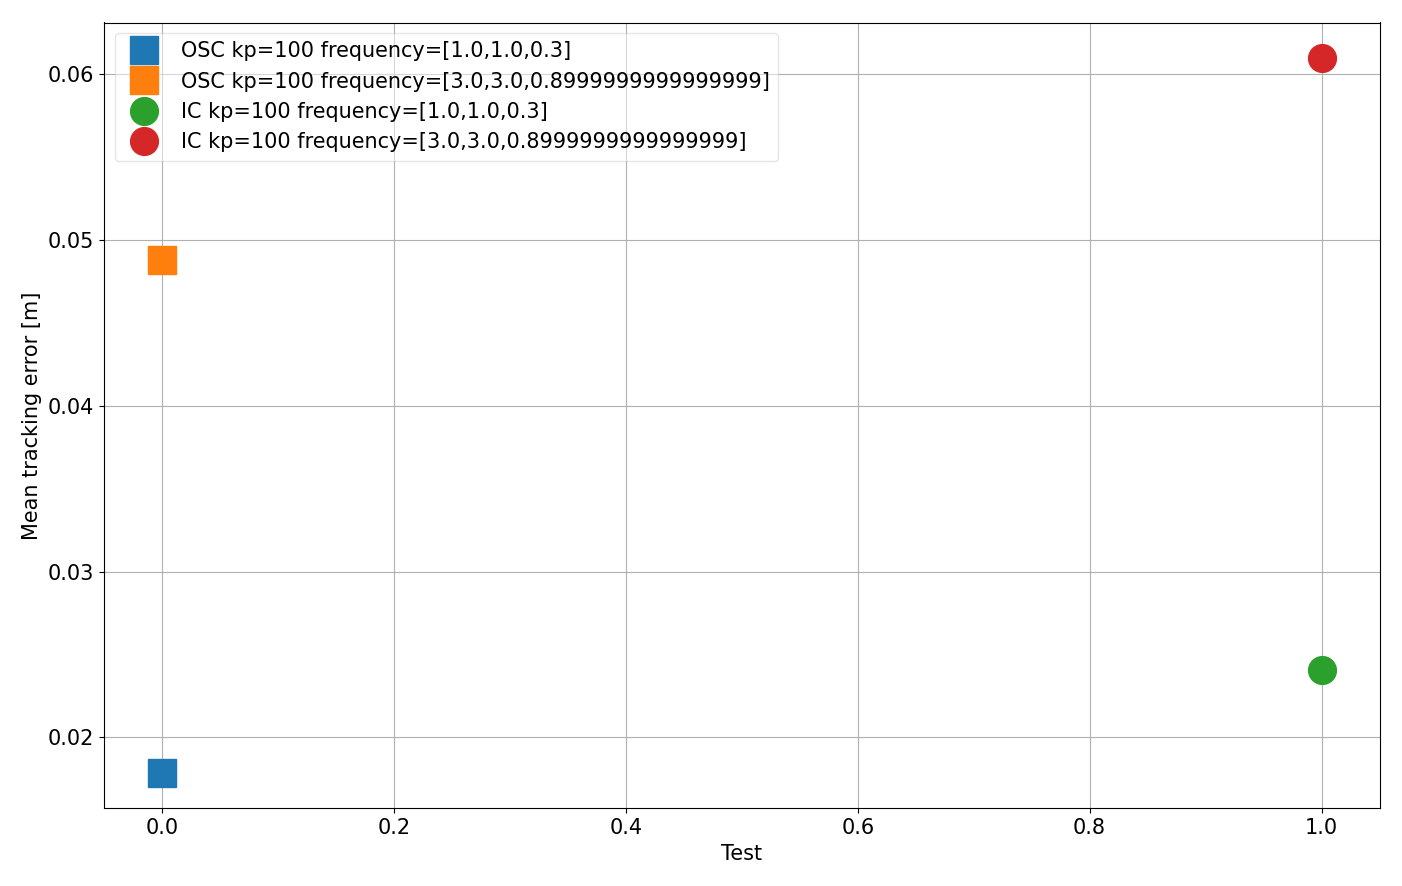
\includegraphics[width=0.5\linewidth]{images/OSCvsIC.png}
    \caption{OSC vs IC}\label{fig:oscvsic}
\end{figure}

\paragraph*{}
The performance of the two control algorithm are slightly different, being the OSC implementation more accurate on the reference trajectory tracking task than the IC implementation.
Thus, when considering the overall performance we can notice that the OSC implementation tends to diverge on joints position, probably due to its prioritization of end effector position.
On the other end, Impedance Control tends to be less strict on end effector position allowing a more stable joint velocities and positions.

\paragraph*{}
At higher frequencies OSC is more accurate on end effector position than IC. The general behavior of IC is more malleable and flexible on end effector position where OSC is more precise.

\paragraph*{}
When increasing the frequency, we also increase the difference between the two algorithms tracking error. We can consider the tracking error difference, between the two implementation, begin proportional to the frequency increment.
But if we experiment with higher frequencies and different robot models we can notice that OSC can be unstable in some cases, while IC tends to produce more consistent results.


\subsection*{Question 2}
\textit{
    Which parameters of the control laws could you tune to improve the controllers performances?
    Re-tune the controllers according to your ideas and report the tracking error obtained.
}

\paragraph*{}
In this example I can try to improve the performance of the controllers by tweaking the value of the proportional gain. I tried increasing the latest to \(500\) achieving a lot better tracking error.
Increasing the proportional gain reduces the effect of the secondary task, leading to unstable joints behavior.
\begin{figure}[h!]
    \centering
    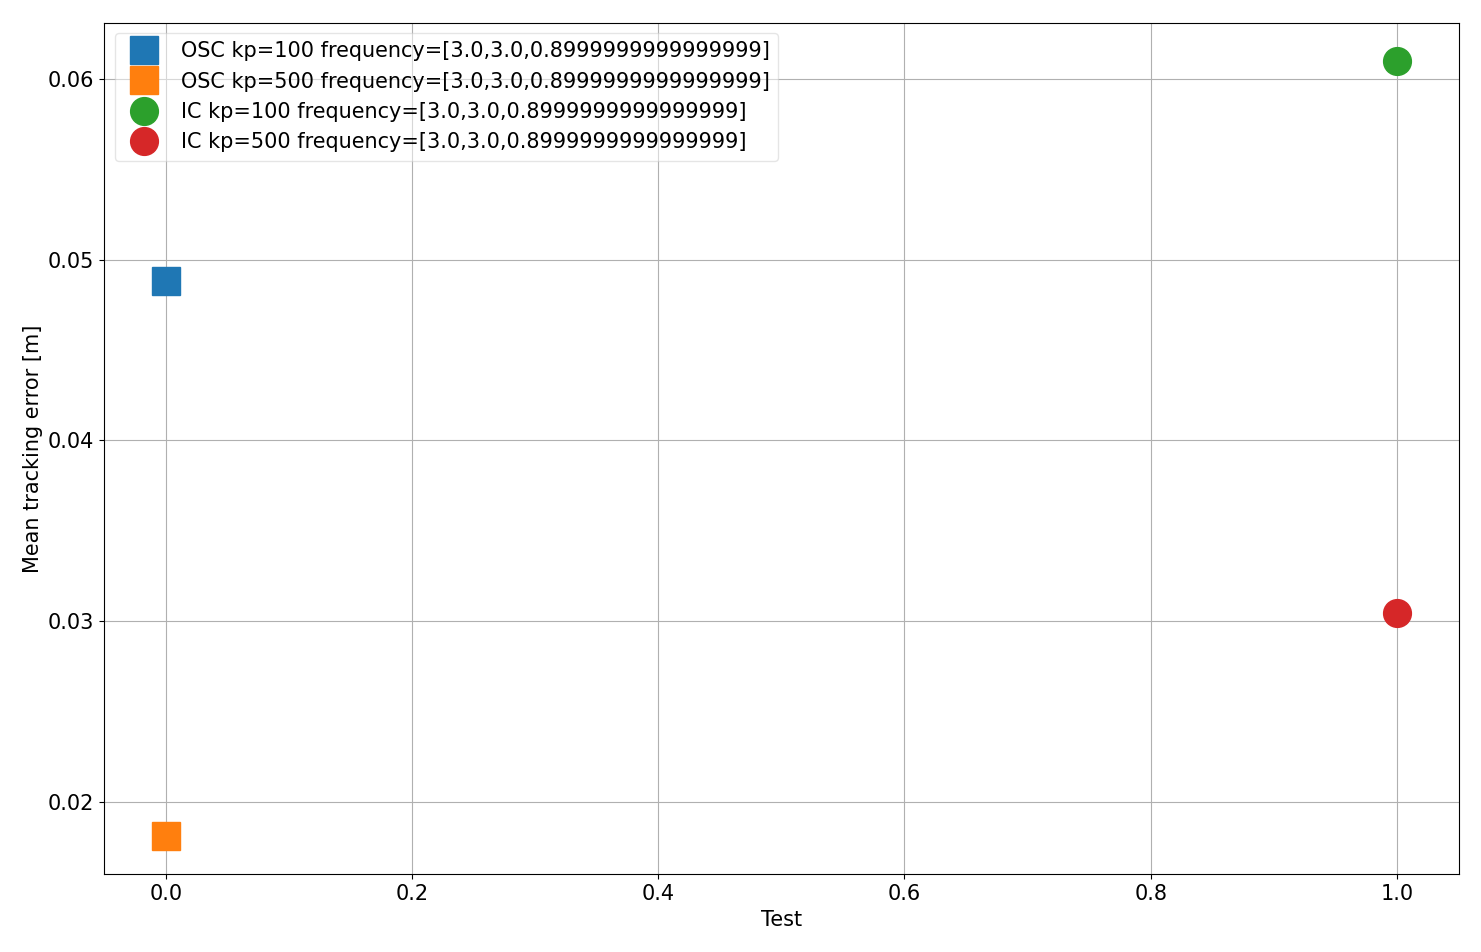
\includegraphics[width=0.5\linewidth]{images/kp_500.png}
    \caption{Increase proportional gain}\label{fig:kp_increase}
\end{figure}

\subsection*{Question 3}
\textit{
    Test the robustness of the controllers to modelling errors by setting to 1 the flag randomize robot model in the configuration file.
    How did the performance of OSC and IC change?
}

\paragraph*{}
At low frequencies the performance of the two control laws does not change much.\\
At higher frequencies on average IC is less accurate on end effector positioning, instead OSC keeps consistent with a law tracking error and stable results.
 
\end{document}